\documentclass[11pt, a4paper]{article}

\usepackage{style}

\author{Vladislav Mlejnecký}

\title{%
  Číslicové zpracování signálů\\
  \large Úloha číslo 12.\\
  Zpracování signálů - korelace - Matlab}

\begin{document}

    \maketitle
    
    \section{Zadání}
    
        \begin{enumerate}
        
            \item 
            \textbf{Korelace - periodický signál} Vygenerujte signál obdélníkovitého průběhu o kmitočtu 300 Hz a délce 100 milisekund.Zvolte
            vzorkovací kmitočet 8000Hz. Pomocí funkce xcorr v Matlabu vypočtěte a nakreslete jejich
            autokorelační funkci.

            \item
            \textbf{Korelace - periodický signál - 2} Vygenerujte signál sinusového průběhu o kmitočtu 200 Hz a délce 100 milisekund.
            Zvolte vzorkovací kmitočet 4000Hz. Pomocí funkce xcorr v Matlabu vypočtěte a nakreslete jeho
            autokorelační funkci. Vypočtěte a nakreslete i vzájemnou korelační funkci.

            \item
            Vypočtěte a nakreslete vzájemnou korelační funkci pro signály dle bodu 1. a 2.

            \item
            Jednotlivé satelity GNSS systémů GPS i Galileo vysílají na stejném kmitočtu. K rozlišení jejich
            signálu se používá tzv. kódový multiplex. Každý satelit má přiřazen jedinečný kód (binární
            posloupnost). Přijímač pak má generátor stejných kódů a shoda generátoru přijímače a kódu ze
            satelitu se zjišťuje pomocí korelační funkce. K detekci satelitu přijímač musí zkoušet známé kódy
            a fáze generátoru, až nalezne maximum korelační funkce.

            Vygenerujte signály (posloupnosti) odpovídající dvěma pseudonáhodným kódům GNSS Galileo
            L1B. Použijte jen část kódu v délce 1023 bitů. Pomocí funkce xcorr v Matlabu vypočtěte a
            nakreslete jejich autokorelační funkce. Vypočtěte a nakreslete i vzájemné korelační funkce.
            Výsledek nakreslete jako dva obrázky pro každou posloupnost, na každém obrázku bude pět
            grafů korelačních funkcí příslušné posloupnosti s ostatními i se sebou.
            
            \item
            Vysvětlete (trojúhelníkovitý) průběh korelační funkce.
        
        \end{enumerate}
        
    \section{Výsledné grafy}
    
            \begin{figure}[H]
                \centering
                \begin{minipage}{.5\textwidth}
                    \centering
                    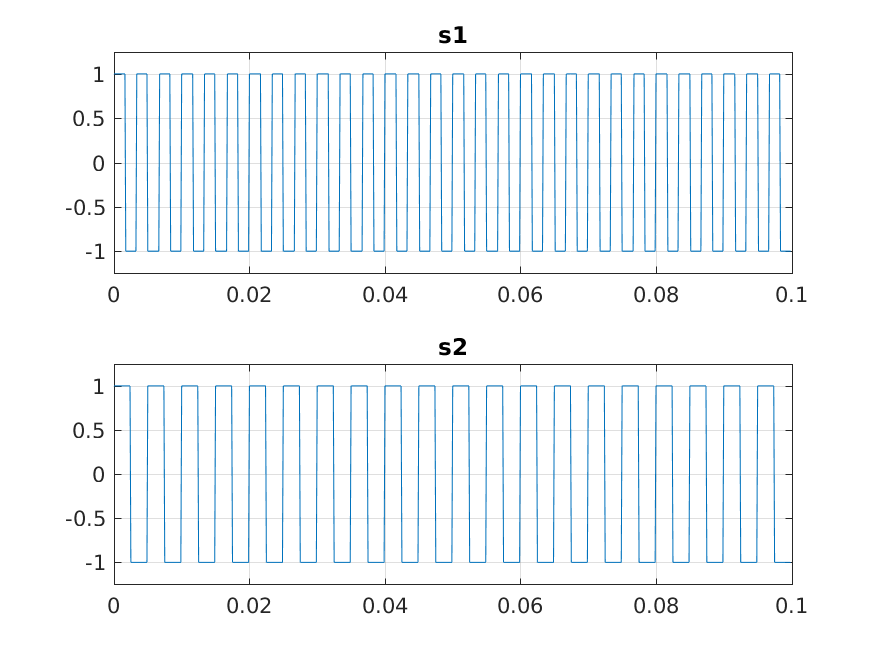
\includegraphics[width=.9\textwidth]{matlab/square_graph.png}
                    \caption{Obdélníkové pulzy}
                    \label{fig:1}
                \end{minipage}%
                \begin{minipage}{.5\textwidth}
                    \centering
                    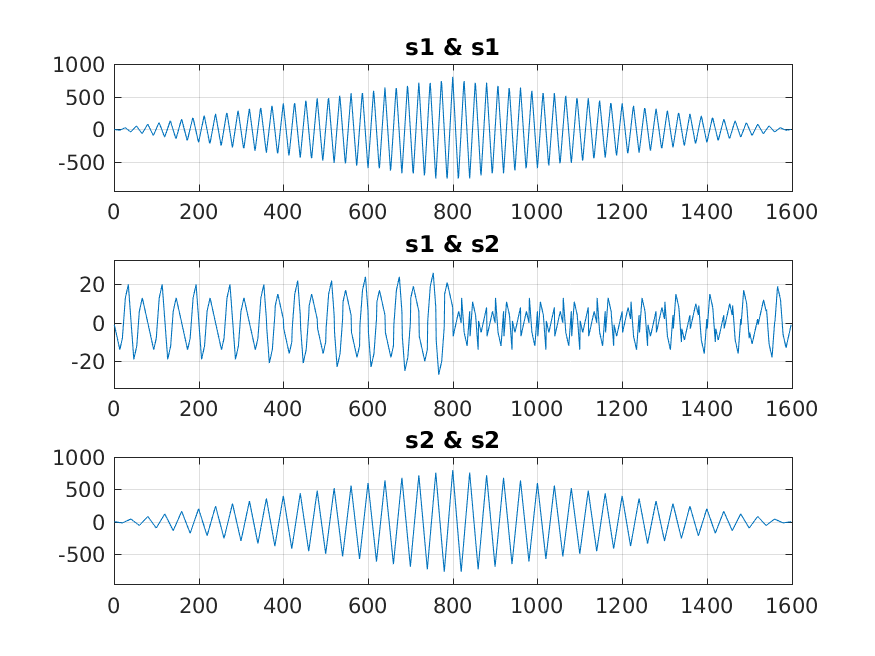
\includegraphics[width=.9\textwidth]{matlab/square_xcorr.png}
                    \caption{Korelace obdélníkových signálů}
                    \label{fig:2}
                \end{minipage}
            \end{figure}

            \begin{figure}[H]
                \centering
                \begin{minipage}{.5\textwidth}
                    \centering
                    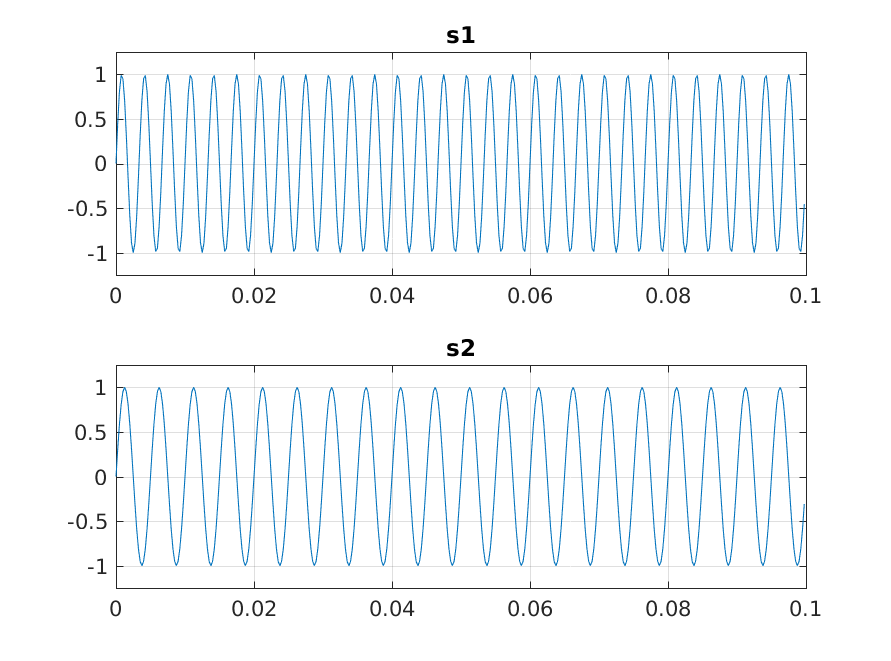
\includegraphics[width=.9\textwidth]{matlab/sine_graph.png}
                    \caption{Sinusové signály}
                    \label{fig:3}
                \end{minipage}%
                \begin{minipage}{.5\textwidth}
                    \centering
                    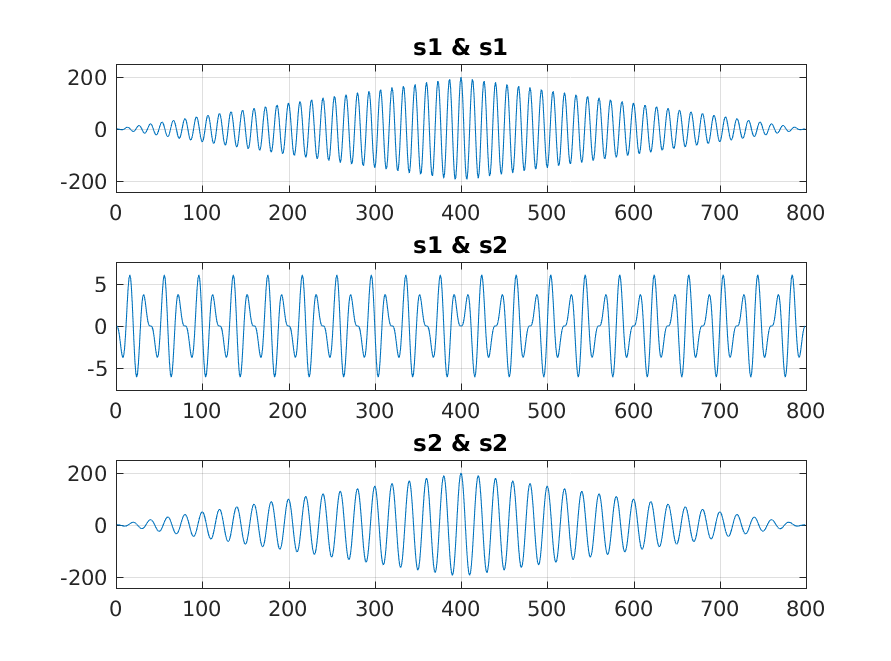
\includegraphics[width=.9\textwidth]{matlab/sine_xcorr.png}
                    \caption{Korelace sinusových signálů}
                    \label{fig:4}
                \end{minipage}
            \end{figure}

            \begin{figure}[H]
                \centering
                \begin{minipage}{.5\textwidth}
                    \centering
                    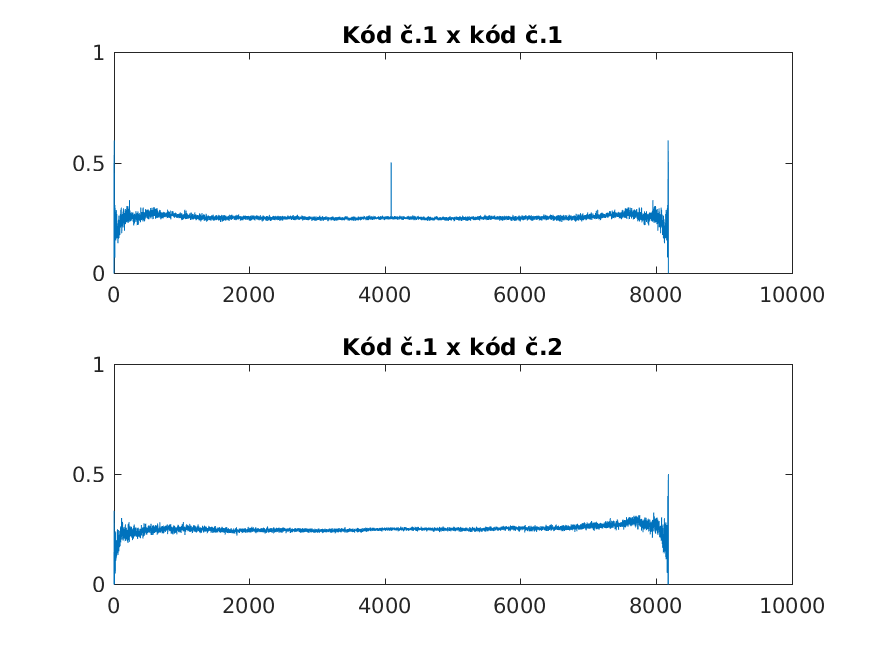
\includegraphics[width=.9\textwidth]{matlab/GPS_1.png}
                    \caption{Korelace signálů GPS 1}
                    \label{fig:5}
                \end{minipage}%
                \begin{minipage}{.5\textwidth}
                    \centering
                    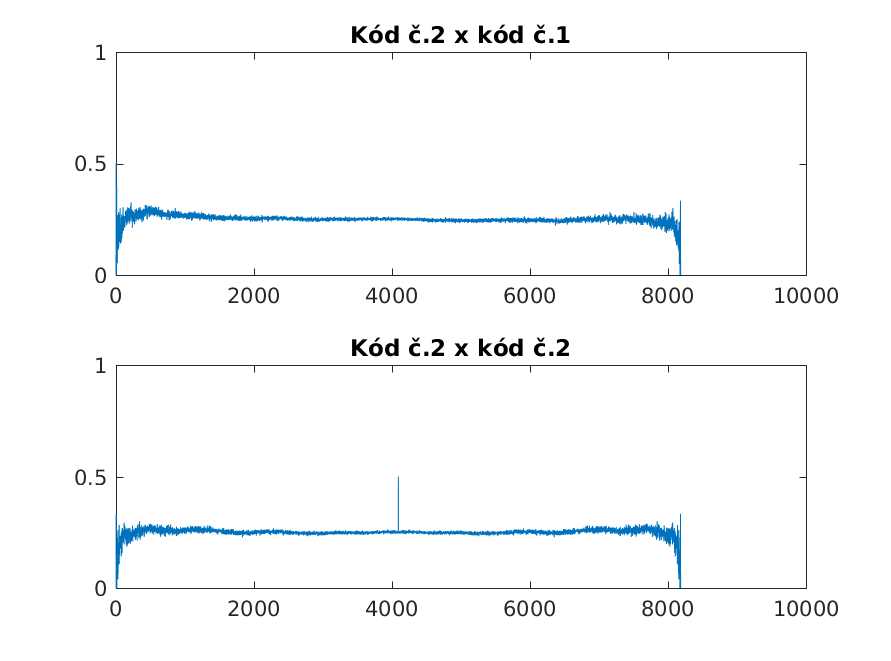
\includegraphics[width=.9\textwidth]{matlab/GPS_2.png}
                    \caption{Korelace signálů GPS 2}
                    \label{fig:6}
                \end{minipage}
            \end{figure}

    
    \section{Výpis zdrojového kódu}
    
\begin{lstlisting}[language=matlab, frame=single] 
ukol1();
ukol2();
ukol3();

function ukol1()
    Fs = 8000;
    t = 0:1/Fs:0.1-1/Fs;

    s1 = square(2*pi*300*t);
    s2 = square(2*pi*200*t);
    
    make_2corr(s1, s2, 'square');
    make_graph(s1, s2, t, 'square');
end

function ukol2()
    Fs = 4000;
    t = 0:1/Fs:0.1-1/Fs;

    s1 = sin(2*pi*300*t);
    s2 = sin(2*pi*200*t);
    
    make_2corr(s1, s2, 'sine');
    make_graph(s1, s2, t, 'sine');
end

function ukol3()
    c=[];
    c(1,:) = strcat('F5D710130573541B9DBD4FD9E9B20A0D59D144C54BC79',...
                    '35539D2E75810FB51E494093A0A19DD79C70C5A98E565',...
                    '7AA578097777E86BCC4651CC72F2F974DC766E07AEA3D',...
                    '0B557EF42FF57E6A58E805358CE9257669133B18F80FD',...
                    'BDFB38C5524C7FB1DE079842482990DF58F72321D9201',...
                    'F8979EAB159B2679C9E95AA6D53456C0DF75C2B4316D1',...
                    'E2309216882854253A1FA60CA2C94ECE013E2A8C94334',...
                    '1E7D9E5A8464B3AD407E0AE465C3E3DD1BE60A8C3D50F',...
                    '831536401E776BE02A6042FC4A27AF653F0CFC4D4D013',...
                    'F115310788D68CAEAD3ECCCC5330587EB3C22A1459FC8',...
                    'E6FCCE9CDE849A5205E70C6D66D125814D698DD0EEBFE',...
                    'AE52CC65C5C84EEDF207379000E169D318426516AC5D1',...
                    'C31F2E18A65E07AE6E33FDD724B13098B3A444688389E',...
                    'FBBB5EEAB588742BB083B679D42FB26FF77919EAB21DE',...
                    '0389D9997498F967AE05AF0F4C7E177416E18C4D5E698',...
                    '7ED3590690AD127D872F14A8F4903A12329732A9768F8',...
                    '2F295BEE391879293E3A97D51435A7F03ED7FBE275F10',...
                    '2A83202DC3DE94AF4C712E9D006D182693E9632933E6E',...
                    'B773880CF147B922E74539E4582F79E39723B4C80E42E',...
                    'DCE4C08A8D02221BAE6D17734817D5B531C0D3C1AE723',...
                    '911F3FFF6AAC02E97FEA69E376AF4761E6451CA61FDB2',...
                    'F9187642EFCD63A09AAB680770C1593EEDD4FF4293BFF',...
                    'D6DD2C3367E85B14A654C834B6699421A');

    c(2,:) = strcat('96B856A629F581D1344FEF597835FE60434625D077ECF',...
                    '0D95FBE1155EA0431979E5AFF544AF591A332FDAEF98A',...
                    'B1EDD847A73F3AF15AAEE7E9A05C9D82C59EC325EF4CF',...
                    '264B8ADF2A8E8BA459354CB4B415CC50BF239ADBC31B3',...
                    'A9C87B0843CF3B9E6D646BA43F866276B053826F3A233',...
                    '4CC5E2EFB9F8F195B382E75EEA63F58A06B3F82A3B5C7',...
                    '7C1800FD9498F803E524435B321210BB84690BED0BBBE',...
                    '16D363B3A90656A73720E27008852FB7DACC8284411B1',...
                    '77728D9527C560859084A395A6F11A96AD9DB6B43E006',...
                    '42B000ED12BFD967868EAB1108552CD4FC89FBC408ACE',...
                    '7678C381EC91DD000319124EB5D5EF52C4CAC9AADEE2F',...
                    'A045C16CE492D7F43743CA77924C78696FCBF2F9F7F36',...
                    'D8E623752200C6FCBBD71ABBB6877F3C5D6E6740AB038',...
                    '9458A6B66440858B2D383244E853646FE2714211DEA9E',...
                    '6196252815BB704A20BFE556AC474F8998944E0CABBBE',...
                    '21A6400B87BFDCF937D12B2821D59298AF4AD378F0F42',...
                    'BD8C41693B8D993CF37C8B478F3BB5D33AD2A9FA24AD7',...
                    'B8FA895FDBC04964192F7BA3FF74E0E3A435B5DFE042E',...
                    '3115CACF29624C0645E9C917534A2EBC1F5665E4E1B1B',...
                    'C56208DBCD8A27CCB6474D5D0E20CA4072C960E5ACE41',...
                    'BDA3770DF3B681F2B318F6F8E1CB17C2857350FB6009A',...
                    'ED665E13B2780D79217F73FAC7A8A48048DB0FB8A8A50',...
                    '07CDDC9A7B2DA8257C99F1CB605A18204');

    pocet = 2;
    x = [];
    for i = 1:pocet
        x2=[];
        for j =1:length(c(i,:))
            x2 = [x2 get_hex2bin(char(upper(c(i,j))))];
        end
        x(i,:)=x2;
    end
    for i = 1:pocet
        h = figure(i);
        for j=1:pocet
           y = xcorr(x(i,:),x(j,:),'unbiased');
           subplot(pocet, 1, j);
           plot(y);
           title(['Kod ' int2str(i) ' x kod ' int2str(j)]);
           ylim([0 1]);
        end
        saveas(h, ['GPS_' int2str(i) '.png']);
        close(h);
    end
end

function y = get_hex2bin(n)
    switch n
        case '0'
            y = [0 0 0 0];
        case '1'
            y = [0 0 0 1];
        case '2'
            y = [0 0 1 0];
        case '3'
            y = [0 0 1 1];
        case '4'
            y = [0 1 0 0];
        case '5'
            y = [0 1 0 1];
        case '6'
            y = [0 1 1 0];
        case '7'
            y = [0 1 1 1];
        case '8'
            y = [1 0 0 0];
        case '9'
            y = [1 0 0 1];
        case 'A'
            y = [1 0 1 0];
        case 'B'
            y = [1 0 1 1];
        case 'C'
            y = [1 1 0 0];
        case 'D'
            y = [1 1 0 1];
        case 'E'
            y = [1 1 1 0];
        case 'F'
            y = [1 1 1 1];
        otherwise
            y = [0 0 0 0];
    end
end

function make_2corr(s1, s2, FileName)
    y1 = xcorr(s1, s1); 
    y2 = xcorr(s1, s2); 
    y3 = xcorr(s2, s2); 

    h = figure(1);
    
    subplot(3,1,1);
    plot(y1);
    title('s1 & s1');
    ylim([(min(y1) - abs(min(y1)/4)) (max(y1) + max(y1)/4)]);
    grid on;
    
    subplot(3,1,2);
    plot(y2);
    title('s1 & s2');
    ylim([(min(y2) - abs(min(y2)/4)) (max(y2) + max(y2)/4)]);
    grid on;
    
    subplot(3,1,3);
    plot(y3);
    title('s2 & s2');
    ylim([(min(y3) - abs(min(y3)/4)) (max(y3) + max(y3)/4)]);
    grid on;
    
    saveas(h, [FileName '_xcorr.png']);
    close(h);
end

function make_graph(s1, s2, t, FileName)
    
    h = figure(1);
    
    subplot(2, 1, 1);
    plot(t, s1);
    ylim([(min(s1) - abs(min(s1)/4)) (max(s1) + max(s1)/4)]);
    title('s1');
    grid on;
    
    subplot(2, 1, 2);
    plot(t, s2);
    ylim([(min(s2) - abs(min(s2)/4)) (max(s2) + max(s2)/4)]);
    title('s2');
    grid on;
    
    saveas(h, [FileName '_graph.png']);
    close(h);
end
\end{lstlisting}

\end{document}
